\subsection{Aufgabenstellung und Versuch}

Für das Subsystem Steuerung mit H-Brücke wurden folgenden Ein- und Ausgänge
definiert.\\

\begin{itemize}
    \item ($In_1$) Die Eingangs- oder Betriebsspannung $U_H$
    \item ($In_2$) Der Momentanstrom $I_{ist}$
    \item ($In_3$) Der angestrebte Strom $I_{soll}$
    \item ($Out_1$) Die Spannung, die über dem Motor abfällt $U_{Motor}$
\end{itemize}


\begin{figure}[H]
    \centering
    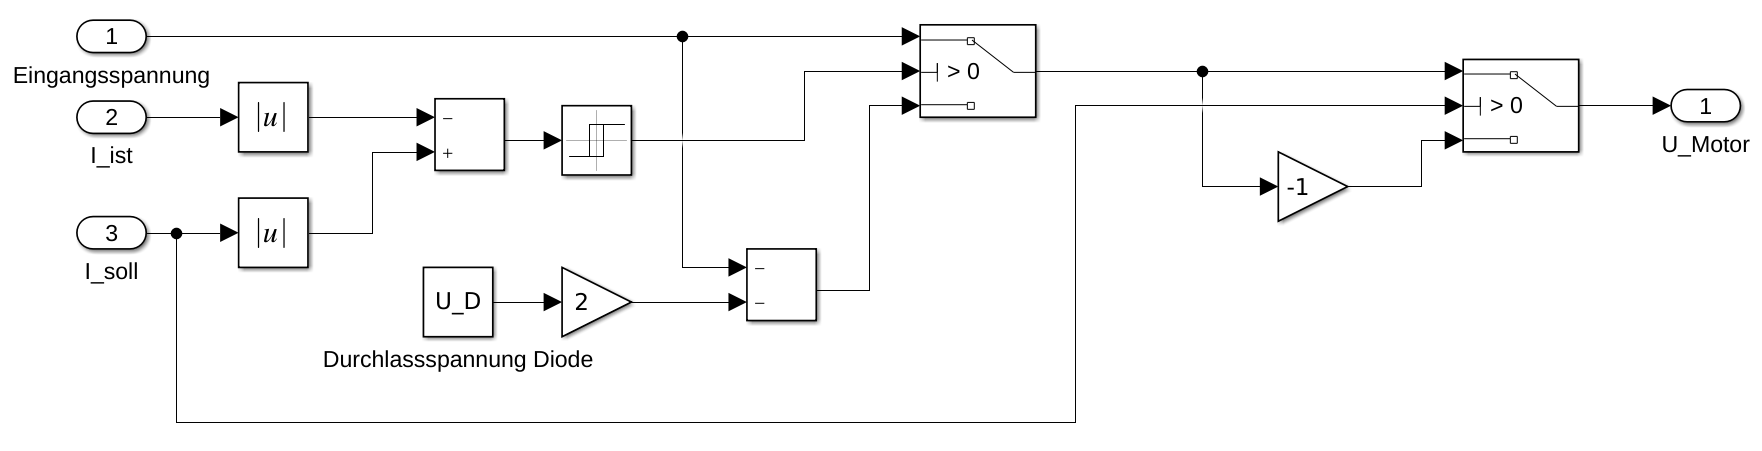
\includegraphics[width=1\textwidth]{hbridge_modell.png}
    \caption{Subsystem Steuerung mit H-Brücke}
    \label{fig:Subsystem H-Bridge}
\end{figure}

Das Subsystem beinhaltet den Relay-Block, der hier als Zweipunktregler genutzt
wird. Die beiden Schwellwerte $i_{plus}=10\mathrm{mA}$ und $i_{minus}=-10
\mathrm{mA}$ wurden im m-File definiert. Der Relay-Block gibt einen boolschen Wert
an den 1. Switch-Block, welcher zwischen Transistoren An und Aus hin- und
herschaltet. Der 2. Switch Block verändert die Drehrichtung des Motors und
wird vom Vorzeichen des einzustellenden Strom $I_{soll}$ geschaltet.

\begin{figure}[H]
    \centering
    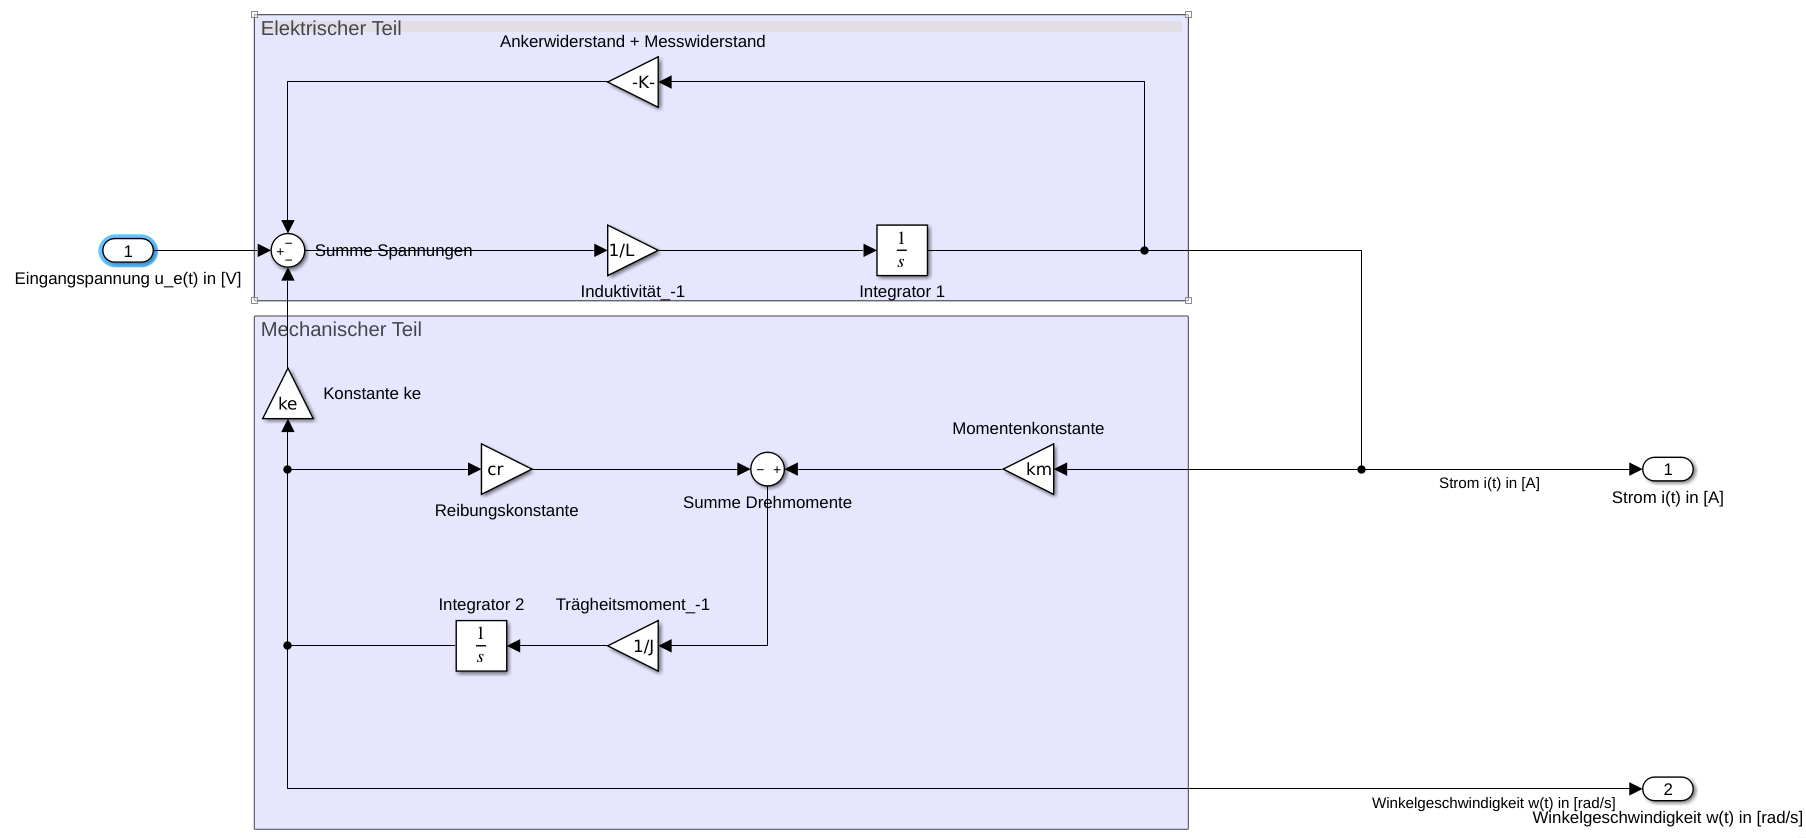
\includegraphics[width=1\textwidth]{dcmotor_modell.png}
    \caption{Subsystem DC-Motor}
    \label{fig:Subsystem DC-Motor}
\end{figure}

Das Subsystem Gleichstrommotor wurde im Labor 3 aufgestellt. Es bekommt
als Eingang eine Eingangspannung $U_M$ und gibt als Ausgang sowohl den
Strom $i_M$ als auch die Winkelgeschwindigkeit $\omega$ zurück.

\begin{figure}[H]
    \centering
    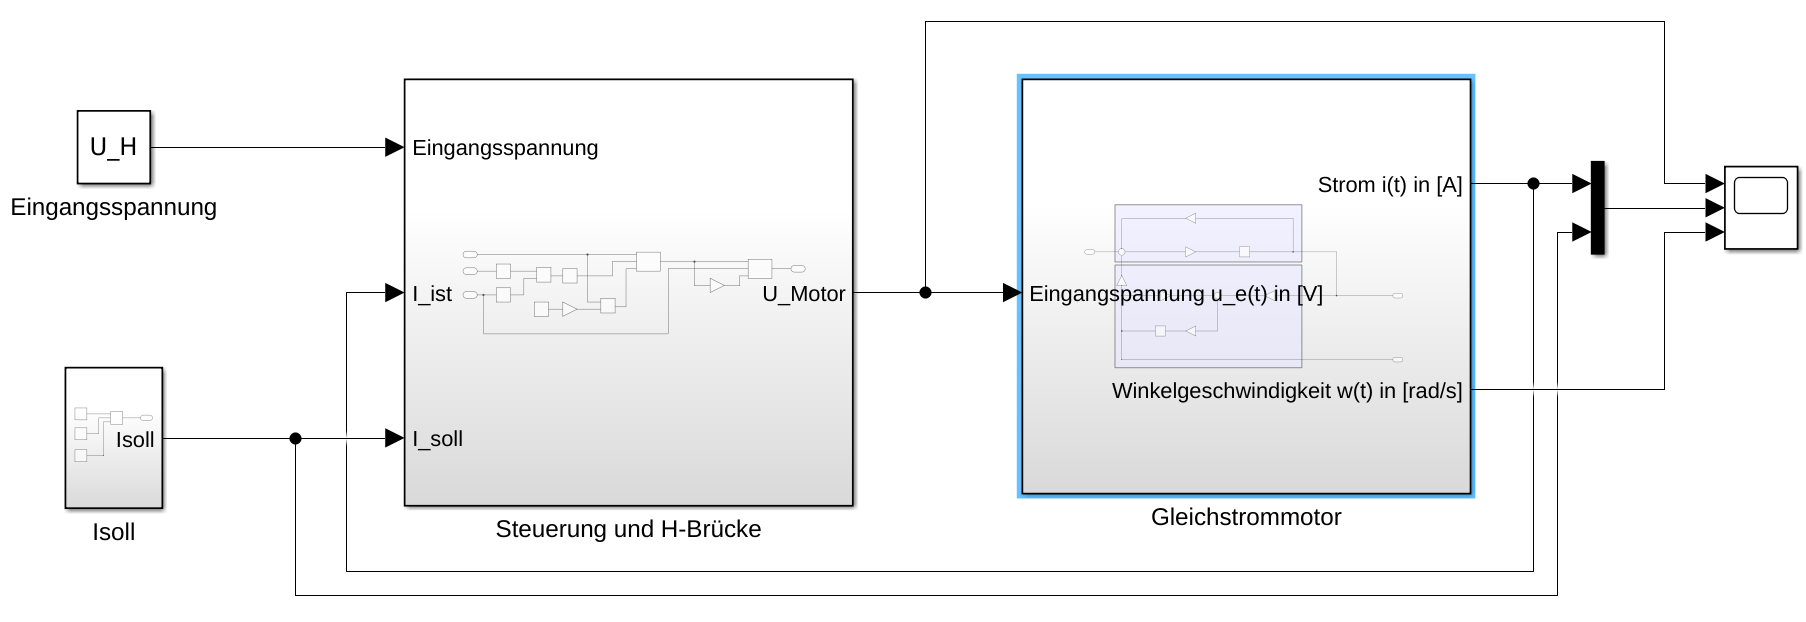
\includegraphics[width=1\textwidth]{hbridge_dcmotor_modell.png}
    \caption{Gesamtsystem}
    \label{fig:Gesamtsystem}
\end{figure}

Das Gesamtsystem besteht aus den beiden vorher beschriebenen Subsystemen, die nun
verbunden werden. Die Eingangspannung $U_H=15\mathrm{V}$ ist im m-file festgelegt.
Im Subblock $I_{soll}$ ist der einzustellende Strom definiert. Dieser beträgt
am Anfang $0.5A$. Nach zwei Sekunden ändert er seinen Wert auf $-0.3A$ und nach
4 Sekunden springt der Strom auf $0.6A$.

Dieses ist gestrichelt in der folgenden Abbildung im mittleren Graph zusehen.
Im selben Graph ist auch der Plot des $I_{ist}$ in rot abgebildet. Im Oberen Graph
ist die gepulste Motorspannung zuerkennen und im unteren Graphen die Winkelgeschwindigkeit.

\begin{figure}[H]
    \centering
    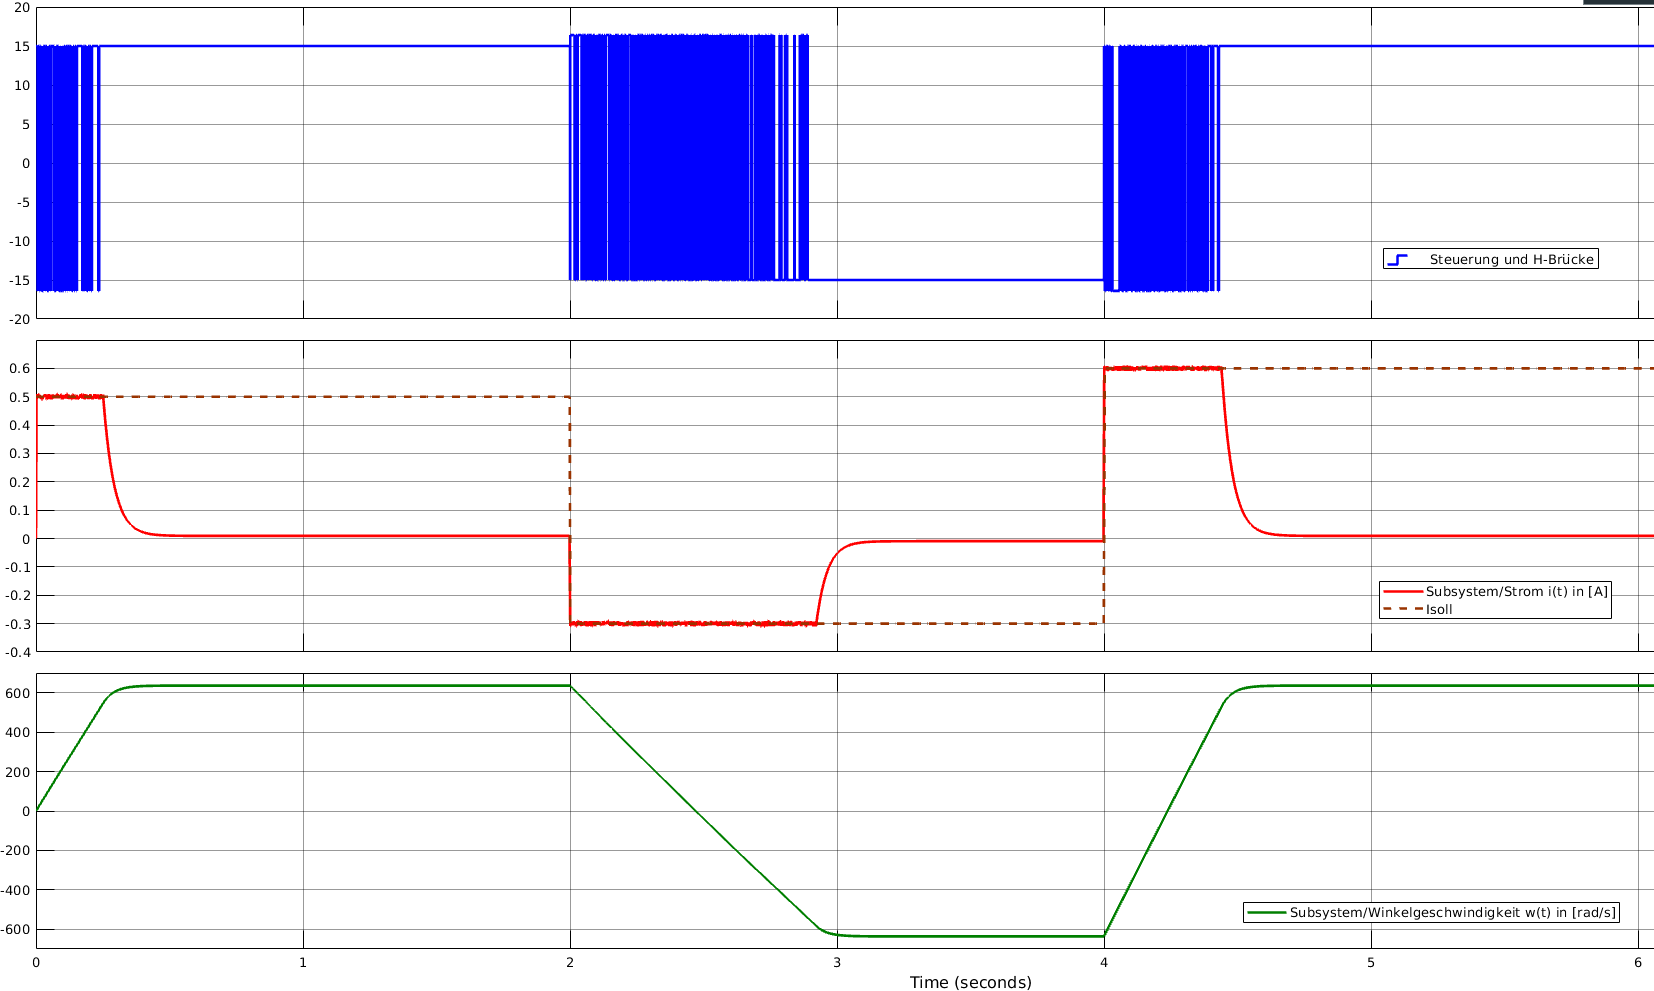
\includegraphics[width=1\textwidth]{hbridge.png}
    \caption{Graph H-Brücke}
    \label{fig:Graph H-Bridge}
\end{figure}

